%%%%%%%%%%%%%%%%%%%%%%%%%%%%%%%%%%%%%%%%%%%%%%%%%%%%%%%%%%%%
% 5.3 MULTIVARIABLE CALCULUS
% The Composition of Advanced Mathematics
%%%%%%%%%%%%%%%%%%%%%%%%%%%%%%%%%%%%%%%%%%%%%%%%%%%%%%%%%%%%

\section{Multivariable Calculus}
\label{sec:multivariable-calculus}

\prerequisite{
Single-variable calculus from \cref{sec:single-variable-calculus},
precalculus and functions from \cref{sec:precalculus-functions},
and basic vector and matrix ideas from \cref{sec:linear-algebra}.
}

\learningobjectives{
By the end of this section, the reader should be able to:
\begin{itemize}
    \item interpret functions of several variables through formulas, level sets, and surfaces;
    \item determine domains of multivariable functions;
    \item understand limits and continuity in several variables;
    \item compute and interpret partial derivatives;
    \item distinguish partial, directional, and total rates of change;
    \item compute gradients and directional derivatives;
    \item interpret the gradient geometrically;
    \item construct tangent planes and linear approximations;
    \item use differentials and the multivariable chain rule;
    \item compute second-order and mixed partial derivatives;
    \item use Hessian matrices to classify critical points;
    \item solve unconstrained and constrained optimization problems;
    \item apply Lagrange multipliers;
    \item evaluate double and triple integrals;
    \item change the order of integration;
    \item use polar, cylindrical, and spherical coordinates;
    \item apply Jacobian factors in changes of variables;
    \item calculate area, volume, mass, center of mass, and average value;
    \item understand the transition from single-variable calculus to higher-dimensional analysis.
\end{itemize}
}

%%%%%%%%%%%%%%%%%%%%%%%%%%%%%%%%%%%%%%%%%%%%%%%%%%%%%%%%%%%%
\subsection{From One Variable to Many}
\label{subsec:from-one-to-many}
%%%%%%%%%%%%%%%%%%%%%%%%%%%%%%%%%%%%%%%%%%%%%%%%%%%%%%%%%%%%

Single-variable calculus studies functions such as

\[ y=f(x). \]

Many mathematical models depend on several independent quantities.

For example, temperature may depend on position:

\[ T=T(x,y,z). \]

Pressure may depend on position and time:

\[ P=P(x,y,z,t). \]

The elevation of a landscape can be modeled by

\[ z=f(x,y). \]

Multivariable calculus extends limits, derivatives, optimization, and
integration to such functions.

\begin{conceptbox}
The essential transition is from motion along a line to behavior throughout
a plane, space, or higher-dimensional domain.
\end{conceptbox}

\begin{center}
\begin{tikzpicture}[
    node distance=12mm and 16mm,
    box/.style={draw,rounded corners,align=center,inner sep=6pt},
    >=stealth
]
\node[box] (one) {One variable\\\(f(x)\)};
\node[box,right=of one] (two) {Two variables\\\(f(x,y)\)};
\node[box,right=of two] (three) {Three variables\\\(f(x,y,z)\)};
\node[box,right=of three] (n) {\(n\) variables\\\(f(x_1,\ldots,x_n)\)};

\draw[->] (one)--(two);
\draw[->] (two)--(three);
\draw[->] (three)--(n);
\end{tikzpicture}
\end{center}

%%%%%%%%%%%%%%%%%%%%%%%%%%%%%%%%%%%%%%%%%%%%%%%%%%%%%%%%%%%%
\subsection{Functions of Several Variables}
\label{subsec:functions-several-variables}
%%%%%%%%%%%%%%%%%%%%%%%%%%%%%%%%%%%%%%%%%%%%%%%%%%%%%%%%%%%%

A real-valued function of two variables may be written

\[ f:D\subseteq\R^2\to\R. \]

This is read:

``\(f\) maps the domain \(D\), contained in \(\R^2\), into the real
numbers.''

Each ordered pair

\[ (x,y)\in D \]

is assigned one real number

\[ z=f(x,y). \]

Similarly,

\[ f:D\subseteq\R^n\to\R \]

represents a real-valued function of \(n\) real variables.

%%%%%%%%%%%%%%%%%%%%%%%%%%%%%%%%%%%%%%%%%%%%%%%%%%%%%%%%%%%%
\subsection{Domains of Multivariable Functions}
\label{subsec:multivariable-domains}
%%%%%%%%%%%%%%%%%%%%%%%%%%%%%%%%%%%%%%%%%%%%%%%%%%%%%%%%%%%%

The domain consists of all input points for which the formula is defined.

Consider

\[ f(x,y)=\sqrt{9-x^2-y^2}. \]

The radicand must satisfy

\[ 9-x^2-y^2\geq0. \]

Therefore,

\[ x^2+y^2\leq9. \]

The domain is the closed disk of radius \(3\) centered at the origin.

\begin{center}
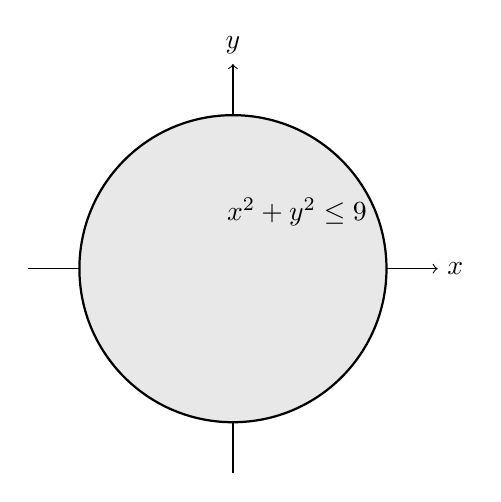
\begin{tikzpicture}[scale=0.65]
\draw[->] (-4,0)--(4,0) node[right] {$x$};
\draw[->] (0,-4)--(0,4) node[above] {$y$};
\fill[gray!18] (0,0) circle (3);
\draw[thick] (0,0) circle (3);
\node at (1.25,1.1) {$x^2+y^2\leq9$};
\end{tikzpicture}
\end{center}

%%%%%%%%%%%%%%%%%%%%%%%%%%%%%%%%%%%%%%%%%%%%%%%%%%%%%%%%%%%%
\subsection{Graphs of Functions of Two Variables}
\label{subsec:graphs-two-variable-functions}
%%%%%%%%%%%%%%%%%%%%%%%%%%%%%%%%%%%%%%%%%%%%%%%%%%%%%%%%%%%%

For

\[ z=f(x,y), \]

the graph is the set

\[ \{(x,y,z)\in\R^3:z=f(x,y)\}. \]

Thus a scalar-valued function of two variables usually produces a surface in
three-dimensional space.

For example,

\[ z=x^2+y^2 \]

is an upward-opening paraboloid.

\begin{center}
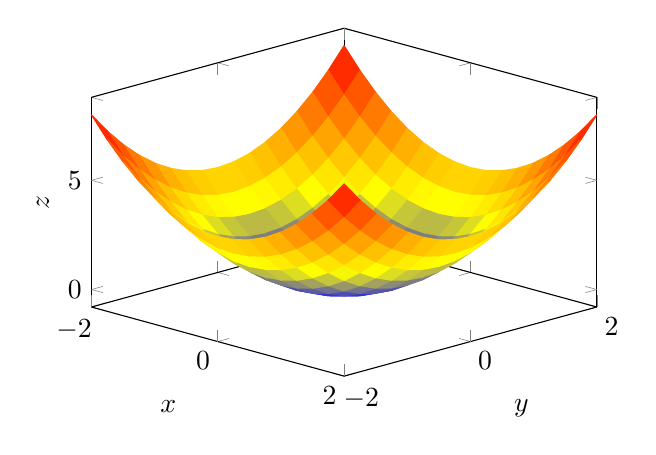
\begin{tikzpicture}
\begin{axis}[
    width=8cm,
    height=6cm,
    view={45}{25},
    xlabel={$x$},
    ylabel={$y$},
    zlabel={$z$},
    domain=-2:2,
    y domain=-2:2
]
\addplot3[surf,shader=flat,samples=17] {x^2+y^2};
\end{axis}
\end{tikzpicture}
\end{center}

%%%%%%%%%%%%%%%%%%%%%%%%%%%%%%%%%%%%%%%%%%%%%%%%%%%%%%%%%%%%
\subsection{Traces}
\label{subsec:multivariable-traces}
%%%%%%%%%%%%%%%%%%%%%%%%%%%%%%%%%%%%%%%%%%%%%%%%%%%%%%%%%%%%

A surface can be studied by intersecting it with vertical or horizontal
planes.

For

\[ z=f(x,y), \]

setting

\[ x=a \]

produces the trace

\[ z=f(a,y). \]

Setting

\[ y=b \]

produces

\[ z=f(x,b). \]

Traces reduce a two-variable function to familiar single-variable curves.

For

\[ z=x^2+y^2, \]

the trace \(y=0\) is

\[ z=x^2, \]

while the trace \(x=0\) is

\[ z=y^2. \]

%%%%%%%%%%%%%%%%%%%%%%%%%%%%%%%%%%%%%%%%%%%%%%%%%%%%%%%%%%%%
\subsection{Level Curves}
\label{subsec:level-curves}
%%%%%%%%%%%%%%%%%%%%%%%%%%%%%%%%%%%%%%%%%%%%%%%%%%%%%%%%%%%%

\begin{definitionbox}{Level Curve}
A \emph{level curve} of a function \(f(x,y)\) is a curve satisfying
\[ f(x,y)=c, \]
where \(c\) is constant.
\end{definitionbox}

Level curves describe locations where a function has the same value.

For

\[ f(x,y)=x^2+y^2, \]

the level curves satisfy

\[ x^2+y^2=c. \]

For \(c>0\), these are circles of radius

\[ \sqrt c. \]

\begin{center}
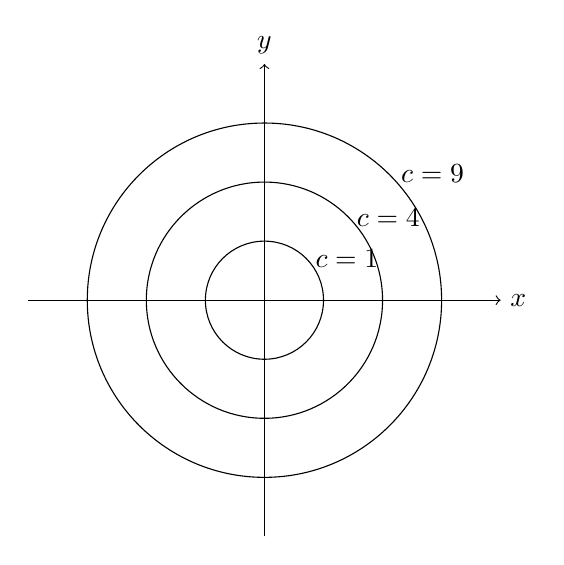
\begin{tikzpicture}[scale=0.75]
\draw[->] (-4,0)--(4,0) node[right] {$x$};
\draw[->] (0,-4)--(0,4) node[above] {$y$};
\draw (0,0) circle (1);
\draw (0,0) circle (2);
\draw (0,0) circle (3);
\node[right] at (0.7,0.7) {$c=1$};
\node[right] at (1.4,1.4) {$c=4$};
\node[right] at (2.15,2.15) {$c=9$};
\end{tikzpicture}
\end{center}

%%%%%%%%%%%%%%%%%%%%%%%%%%%%%%%%%%%%%%%%%%%%%%%%%%%%%%%%%%%%
\subsection{Contour Maps}
\label{subsec:contour-maps}
%%%%%%%%%%%%%%%%%%%%%%%%%%%%%%%%%%%%%%%%%%%%%%%%%%%%%%%%%%%%

A collection of level curves is called a \emph{contour map}.

Contour maps encode three-dimensional information in two dimensions.

Common examples include:

\begin{itemize}
    \item elevation maps;
    \item temperature maps;
    \item pressure maps;
    \item concentration maps;
    \item potential-energy diagrams.
\end{itemize}

Closely spaced level curves often indicate rapid change, while widely spaced
curves indicate slower change.

%%%%%%%%%%%%%%%%%%%%%%%%%%%%%%%%%%%%%%%%%%%%%%%%%%%%%%%%%%%%
\subsection{Level Surfaces}
\label{subsec:level-surfaces}
%%%%%%%%%%%%%%%%%%%%%%%%%%%%%%%%%%%%%%%%%%%%%%%%%%%%%%%%%%%%

For a function of three variables

\[ F(x,y,z), \]

an equation

\[ F(x,y,z)=c \]

defines a \emph{level surface}.

For example,

\[ F(x,y,z)=x^2+y^2+z^2 \]

has level surfaces

\[ x^2+y^2+z^2=c. \]

For \(c>0\), these are spheres of radius \(\sqrt c\).

%%%%%%%%%%%%%%%%%%%%%%%%%%%%%%%%%%%%%%%%%%%%%%%%%%%%%%%%%%%%
\subsection{Limits in Several Variables}
\label{subsec:multivariable-limits}
%%%%%%%%%%%%%%%%%%%%%%%%%%%%%%%%%%%%%%%%%%%%%%%%%%%%%%%%%%%%

The notation

\[ \lim_{(x,y)\to(a,b)}f(x,y)=L \]

is read:

``the limit of \(f(x,y)\) as \((x,y)\) approaches \((a,b)\) is \(L\).''

Unlike the single-variable case, a point in the plane can be approached
along infinitely many paths.

For a limit to exist, the function must approach the same value along
\emph{every} possible path.

%%%%%%%%%%%%%%%%%%%%%%%%%%%%%%%%%%%%%%%%%%%%%%%%%%%%%%%%%%%%
\subsection{Path Dependence}
\label{subsec:path-dependence}
%%%%%%%%%%%%%%%%%%%%%%%%%%%%%%%%%%%%%%%%%%%%%%%%%%%%%%%%%%%%

Consider

\[ f(x,y)=\frac{x^2-y^2}{x^2+y^2}. \]

Approach \((0,0)\) along

\[ y=0. \]

Then

\[ f(x,0)=1. \]

Hence

\[ \lim_{x\to0}f(x,0)=1. \]

Approach instead along

\[ x=0. \]

Then

\[ f(0,y)=-1. \]

Therefore,

\[ \lim_{y\to0}f(0,y)=-1. \]

Since the path limits disagree,

\[ \boxed{\lim_{(x,y)\to(0,0)}
\frac{x^2-y^2}{x^2+y^2}\text{ does not exist}.} \]

%%%%%%%%%%%%%%%%%%%%%%%%%%%%%%%%%%%%%%%%%%%%%%%%%%%%%%%%%%%%
\subsection{Path Testing and Its Limitation}
\label{subsec:path-testing-limitation}
%%%%%%%%%%%%%%%%%%%%%%%%%%%%%%%%%%%%%%%%%%%%%%%%%%%%%%%%%%%%

Finding two paths with different limiting values proves that a multivariable
limit does not exist.

However, checking several paths that give the same value does \emph{not}
prove that the limit exists.

\begin{warningbox}
Path testing is powerful for disproving limits but usually insufficient for
proving them.
\end{warningbox}

To prove existence, one generally needs inequalities, comparison arguments,
coordinate transformations, or the formal multivariable limit definition.

%%%%%%%%%%%%%%%%%%%%%%%%%%%%%%%%%%%%%%%%%%%%%%%%%%%%%%%%%%%%
\subsection{Polar Coordinates and Limits}
\label{subsec:polar-limits}
%%%%%%%%%%%%%%%%%%%%%%%%%%%%%%%%%%%%%%%%%%%%%%%%%%%%%%%%%%%%

Near the origin, substitutions

\[ x=r\cos\theta,\qquad y=r\sin\theta \]

can simplify limits because

\[ x^2+y^2=r^2. \]

The Greek letter

\[ \theta \]

is theta, commonly pronounced ``THAY-tuh.''

Here \(\theta\) represents an angle.

As

\[ (x,y)\to(0,0), \]

we have

\[ r\to0. \]

If the resulting expression approaches a value independent of \(\theta\),
this often helps establish the limit.

%%%%%%%%%%%%%%%%%%%%%%%%%%%%%%%%%%%%%%%%%%%%%%%%%%%%%%%%%%%%
\subsection{Worked Example: A Multivariable Limit}
\label{subsec:worked-multivariable-limit}
%%%%%%%%%%%%%%%%%%%%%%%%%%%%%%%%%%%%%%%%%%%%%%%%%%%%%%%%%%%%

\begin{workedexamplebox}{Using Polar Coordinates}

Evaluate

\[ \lim_{(x,y)\to(0,0)}
\frac{x^2y^2}{x^2+y^2}. \]

\begin{tabularx}{\textwidth}{@{}>{\raggedright\arraybackslash}p{0.42\textwidth}X@{}}
Use polar coordinates. &
\(x=r\cos\theta,\quad y=r\sin\theta\)\\
Rewrite the numerator. &
\(x^2y^2=r^4\cos^2\theta\sin^2\theta\)\\
Rewrite the denominator. &
\(x^2+y^2=r^2\)\\
Simplify. &
\(r^2\cos^2\theta\sin^2\theta\)\\
Use boundedness of the trigonometric factors. &
\(\left|r^2\cos^2\theta\sin^2\theta\right|\leq r^2\)\\
Let \(r\to0\). &
\(r^2\to0\)
\end{tabularx}

\begin{answerbox}
\[ \boxed{\lim_{(x,y)\to(0,0)}
\frac{x^2y^2}{x^2+y^2}=0.} \]
\end{answerbox}
\end{workedexamplebox}

%%%%%%%%%%%%%%%%%%%%%%%%%%%%%%%%%%%%%%%%%%%%%%%%%%%%%%%%%%%%
\subsection{Continuity in Several Variables}
\label{subsec:multivariable-continuity}
%%%%%%%%%%%%%%%%%%%%%%%%%%%%%%%%%%%%%%%%%%%%%%%%%%%%%%%%%%%%

\begin{definitionbox}{Continuity at a Point}
A function \(f(x,y)\) is continuous at \((a,b)\) if
\[ \lim_{(x,y)\to(a,b)}f(x,y)=f(a,b). \]
\end{definitionbox}

As in single-variable calculus, continuity requires:

\begin{enumerate}
    \item the function value to exist;
    \item the limit to exist;
    \item the two values to agree.
\end{enumerate}

Polynomials in several variables are continuous everywhere.

Rational functions are continuous wherever their denominators are nonzero.

%%%%%%%%%%%%%%%%%%%%%%%%%%%%%%%%%%%%%%%%%%%%%%%%%%%%%%%%%%%%
\subsection{Partial Derivatives}
\label{subsec:partial-derivatives}
%%%%%%%%%%%%%%%%%%%%%%%%%%%%%%%%%%%%%%%%%%%%%%%%%%%%%%%%%%%%

For

\[ z=f(x,y), \]

we may ask how \(z\) changes as \(x\) changes while \(y\) is held fixed.

This produces the partial derivative with respect to \(x\).

\begin{definitionbox}{Partial Derivative with Respect to \(x\)}
The partial derivative of \(f\) with respect to \(x\) is
\[ f_x(x,y)=\frac{\partial f}{\partial x}
=\lim_{h\to0}\frac{f(x+h,y)-f(x,y)}{h}, \]
provided the limit exists.
\end{definitionbox}

The symbol

\[ \partial \]

is called the \emph{partial derivative symbol} and is commonly pronounced
``partial.''

Thus

\[ \frac{\partial f}{\partial x} \]

is read:

``the partial derivative of \(f\) with respect to \(x\).''

Similarly,

\[ f_y(x,y)=\frac{\partial f}{\partial y}. \]

%%%%%%%%%%%%%%%%%%%%%%%%%%%%%%%%%%%%%%%%%%%%%%%%%%%%%%%%%%%%
\subsection{Computing Partial Derivatives}
\label{subsec:computing-partials}
%%%%%%%%%%%%%%%%%%%%%%%%%%%%%%%%%%%%%%%%%%%%%%%%%%%%%%%%%%%%

To compute

\[ f_x, \]

treat \(y\) as a constant.

To compute

\[ f_y, \]

treat \(x\) as a constant.

For

\[ f(x,y)=x^2y+3xy^2, \]

we obtain

\[ f_x(x,y)=2xy+3y^2, \]

and

\[ f_y(x,y)=x^2+6xy. \]

%%%%%%%%%%%%%%%%%%%%%%%%%%%%%%%%%%%%%%%%%%%%%%%%%%%%%%%%%%%%
\subsection{Worked Example: Partial Derivatives}
\label{subsec:worked-partials}
%%%%%%%%%%%%%%%%%%%%%%%%%%%%%%%%%%%%%%%%%%%%%%%%%%%%%%%%%%%%

\begin{workedexamplebox}{Computing First Partial Derivatives}

Let

\[ f(x,y)=x^3y^2+e^{xy}. \]

Find \(f_x\) and \(f_y\).

\begin{tabularx}{\textwidth}{@{}>{\raggedright\arraybackslash}p{0.42\textwidth}X@{}}
Differentiate with respect to \(x\), treating \(y\) as constant. &
\(f_x=3x^2y^2+ye^{xy}\)\\
Differentiate with respect to \(y\), treating \(x\) as constant. &
\(f_y=2x^3y+xe^{xy}\)
\end{tabularx}

\begin{answerbox}
\[ \boxed{f_x=3x^2y^2+ye^{xy},\qquad
f_y=2x^3y+xe^{xy}.} \]
\end{answerbox}
\end{workedexamplebox}

%%%%%%%%%%%%%%%%%%%%%%%%%%%%%%%%%%%%%%%%%%%%%%%%%%%%%%%%%%%%
\subsection{Geometric Meaning of Partial Derivatives}
\label{subsec:geometric-partials}
%%%%%%%%%%%%%%%%%%%%%%%%%%%%%%%%%%%%%%%%%%%%%%%%%%%%%%%%%%%%

For a surface

\[ z=f(x,y), \]

the derivative

\[ f_x(a,b) \]

is the slope of the tangent line to the trace obtained by fixing

\[ y=b. \]

Similarly,

\[ f_y(a,b) \]

is the tangent slope obtained by fixing

\[ x=a. \]

Thus partial derivatives measure change along the coordinate directions.

%%%%%%%%%%%%%%%%%%%%%%%%%%%%%%%%%%%%%%%%%%%%%%%%%%%%%%%%%%%%
\subsection{Partial Derivatives in Higher Dimensions}
\label{subsec:higher-dimensional-partials}
%%%%%%%%%%%%%%%%%%%%%%%%%%%%%%%%%%%%%%%%%%%%%%%%%%%%%%%%%%%%

For

\[ f(x_1,x_2,\ldots,x_n), \]

there is one first partial derivative for each input variable:

\[ \frac{\partial f}{\partial x_1},
\frac{\partial f}{\partial x_2},
\ldots,
\frac{\partial f}{\partial x_n}. \]

Each measures change in one coordinate direction while the remaining
coordinates are held fixed.

%%%%%%%%%%%%%%%%%%%%%%%%%%%%%%%%%%%%%%%%%%%%%%%%%%%%%%%%%%%%
\subsection{Second Partial Derivatives}
\label{subsec:second-partials}
%%%%%%%%%%%%%%%%%%%%%%%%%%%%%%%%%%%%%%%%%%%%%%%%%%%%%%%%%%%%

Partial derivatives can themselves be differentiated.

For \(f(x,y)\), the second partial derivatives are

\[ f_{xx},\qquad f_{xy},\qquad f_{yx},\qquad f_{yy}. \]

For example,

\[ f_{xy}
=\frac{\partial}{\partial y}
\left(\frac{\partial f}{\partial x}\right). \]

The derivatives \(f_{xy}\) and \(f_{yx}\) are called \emph{mixed partial
derivatives}.

%%%%%%%%%%%%%%%%%%%%%%%%%%%%%%%%%%%%%%%%%%%%%%%%%%%%%%%%%%%%
\subsection{Equality of Mixed Partials}
\label{subsec:equality-mixed-partials}
%%%%%%%%%%%%%%%%%%%%%%%%%%%%%%%%%%%%%%%%%%%%%%%%%%%%%%%%%%%%

\begin{theorem}[Clairaut's Theorem]
If the relevant second partial derivatives are continuous near a point, then
\[ f_{xy}=f_{yx}. \]
\end{theorem}

Thus, under suitable regularity conditions, the order of differentiation
does not matter.

%%%%%%%%%%%%%%%%%%%%%%%%%%%%%%%%%%%%%%%%%%%%%%%%%%%%%%%%%%%%
\subsection{Differentiability}
\label{subsec:multivariable-differentiability}
%%%%%%%%%%%%%%%%%%%%%%%%%%%%%%%%%%%%%%%%%%%%%%%%%%%%%%%%%%%%

In one variable, differentiability means that a function is locally
approximated by a line.

In two variables, differentiability means that a function is locally
approximated by a plane.

This is stronger than merely having partial derivatives.

\begin{warningbox}
The existence of \(f_x(a,b)\) and \(f_y(a,b)\) alone does not guarantee that
\(f\) is differentiable at \((a,b)\).
\end{warningbox}

A useful sufficient condition is that the first partial derivatives exist
and are continuous in a neighborhood of the point.

%%%%%%%%%%%%%%%%%%%%%%%%%%%%%%%%%%%%%%%%%%%%%%%%%%%%%%%%%%%%
\subsection{Tangent Planes}
\label{subsec:tangent-planes}
%%%%%%%%%%%%%%%%%%%%%%%%%%%%%%%%%%%%%%%%%%%%%%%%%%%%%%%%%%%%

For

\[ z=f(x,y), \]

the tangent plane at

\[ (a,b,f(a,b)) \]

is

\[ \boxed{
z-f(a,b)
=
f_x(a,b)(x-a)
+
f_y(a,b)(y-b).
} \]

This is the multivariable analogue of the tangent-line equation

\[ y-f(a)=f'(a)(x-a). \]

%%%%%%%%%%%%%%%%%%%%%%%%%%%%%%%%%%%%%%%%%%%%%%%%%%%%%%%%%%%%
\subsection{Linearization}
\label{subsec:multivariable-linearization}
%%%%%%%%%%%%%%%%%%%%%%%%%%%%%%%%%%%%%%%%%%%%%%%%%%%%%%%%%%%%

The linearization of \(f(x,y)\) at \((a,b)\) is

\[ L(x,y)
=
f(a,b)
+
f_x(a,b)(x-a)
+
f_y(a,b)(y-b). \]

For points near \((a,b)\),

\[ f(x,y)\approx L(x,y). \]

The tangent plane is therefore the best first-order linear approximation to
the surface near the point.

%%%%%%%%%%%%%%%%%%%%%%%%%%%%%%%%%%%%%%%%%%%%%%%%%%%%%%%%%%%%
\subsection{Worked Example: Tangent Plane}
\label{subsec:worked-tangent-plane}
%%%%%%%%%%%%%%%%%%%%%%%%%%%%%%%%%%%%%%%%%%%%%%%%%%%%%%%%%%%%

\begin{workedexamplebox}{Finding a Tangent Plane}

Find the tangent plane to

\[ z=x^2+xy+y^2 \]

at \((1,1,3)\).

\begin{tabularx}{\textwidth}{@{}>{\raggedright\arraybackslash}p{0.42\textwidth}X@{}}
Compute \(f_x\). &
\(f_x=2x+y\)\\
Evaluate at \((1,1)\). &
\(f_x(1,1)=3\)\\
Compute \(f_y\). &
\(f_y=x+2y\)\\
Evaluate at \((1,1)\). &
\(f_y(1,1)=3\)\\
Use the tangent-plane formula. &
\(z-3=3(x-1)+3(y-1)\)
\end{tabularx}

\begin{answerbox}
\[ \boxed{z=3x+3y-3.} \]
\end{answerbox}
\end{workedexamplebox}

%%%%%%%%%%%%%%%%%%%%%%%%%%%%%%%%%%%%%%%%%%%%%%%%%%%%%%%%%%%%
\subsection{Differentials}
\label{subsec:multivariable-differentials}
%%%%%%%%%%%%%%%%%%%%%%%%%%%%%%%%%%%%%%%%%%%%%%%%%%%%%%%%%%%%

For

\[ z=f(x,y), \]

the total differential is

\[ dz=f_x\,dx+f_y\,dy. \]

For small changes \(\Delta x\) and \(\Delta y\),

\[ \Delta z\approx dz. \]

Thus

\[ \Delta z
\approx
f_x\Delta x+f_y\Delta y. \]

This provides a practical method for approximation and error estimation.

%%%%%%%%%%%%%%%%%%%%%%%%%%%%%%%%%%%%%%%%%%%%%%%%%%%%%%%%%%%%
\subsection{The Gradient}
\label{subsec:gradient}
%%%%%%%%%%%%%%%%%%%%%%%%%%%%%%%%%%%%%%%%%%%%%%%%%%%%%%%%%%%%

The first partial derivatives can be collected into a vector.

\begin{definitionbox}{Gradient}
For a scalar-valued function
\[ f:\R^n\to\R, \]
the \emph{gradient} is
\[ \nabla f
=
\left\langle
\frac{\partial f}{\partial x_1},
\ldots,
\frac{\partial f}{\partial x_n}
\right\rangle.
\]
\end{definitionbox}

The symbol

\[ \nabla \]

is called \emph{nabla} or \emph{del}.

It is commonly read ``grad'' when used in the expression

\[ \nabla f, \]

which is read ``the gradient of \(f\).''

For

\[ f(x,y), \]

\[ \nabla f=\langle f_x,f_y\rangle. \]

%%%%%%%%%%%%%%%%%%%%%%%%%%%%%%%%%%%%%%%%%%%%%%%%%%%%%%%%%%%%
\subsection{Directional Derivatives}
\label{subsec:directional-derivatives}
%%%%%%%%%%%%%%%%%%%%%%%%%%%%%%%%%%%%%%%%%%%%%%%%%%%%%%%%%%%%

Partial derivatives measure change only in coordinate directions.

A directional derivative measures change in any chosen direction.

Let

\[ \vect{u}=\langle u_1,u_2\rangle \]

be a unit vector.

\begin{definitionbox}{Directional Derivative}
The directional derivative of \(f\) in the direction \(\vect{u}\) is
\[ D_{\vect{u}}f
=
\nabla f\cdot\vect{u}. \]
\end{definitionbox}

The notation

\[ D_{\vect{u}}f \]

is read:

``the directional derivative of \(f\) in the direction \(\vect{u}\).''

%%%%%%%%%%%%%%%%%%%%%%%%%%%%%%%%%%%%%%%%%%%%%%%%%%%%%%%%%%%%
\subsection{Worked Example: Directional Derivative}
\label{subsec:worked-directional-derivative}
%%%%%%%%%%%%%%%%%%%%%%%%%%%%%%%%%%%%%%%%%%%%%%%%%%%%%%%%%%%%

\begin{workedexamplebox}{Change in a Given Direction}

Let

\[ f(x,y)=x^2+3y^2. \]

Find the directional derivative at \((1,2)\) in the direction of

\[ \vect{v}=\langle3,4\rangle. \]

\begin{tabularx}{\textwidth}{@{}>{\raggedright\arraybackslash}p{0.42\textwidth}X@{}}
Compute the gradient. &
\(\nabla f=\langle2x,6y\rangle\)\\
Evaluate at the point. &
\(\nabla f(1,2)=\langle2,12\rangle\)\\
Normalize the direction vector. &
\(\displaystyle \vect{u}=\left\langle\frac35,\frac45\right\rangle\)\\
Take the dot product. &
\(\displaystyle D_{\vect{u}}f
=\langle2,12\rangle\cdot
\left\langle\frac35,\frac45\right\rangle\)\\
Simplify. &
\(\displaystyle D_{\vect{u}}f=\frac{54}{5}\)
\end{tabularx}

\begin{answerbox}
\[ \boxed{D_{\vect{u}}f(1,2)=\frac{54}{5}.} \]
\end{answerbox}
\end{workedexamplebox}

%%%%%%%%%%%%%%%%%%%%%%%%%%%%%%%%%%%%%%%%%%%%%%%%%%%%%%%%%%%%
\subsection{Direction of Maximum Increase}
\label{subsec:maximum-increase-gradient}
%%%%%%%%%%%%%%%%%%%%%%%%%%%%%%%%%%%%%%%%%%%%%%%%%%%%%%%%%%%%

Since

\[ D_{\vect{u}}f=\nabla f\cdot\vect{u}, \]

the dot-product formula gives

\[ D_{\vect{u}}f
=
\norm{\nabla f}\norm{\vect{u}}\cos\theta. \]

For a unit vector,

\[ \norm{\vect{u}}=1. \]

Therefore,

\[ D_{\vect{u}}f=\norm{\nabla f}\cos\theta. \]

The maximum occurs when

\[ \theta=0. \]

Thus:

\begin{importantbox}
The gradient points in the direction of greatest increase of \(f\), and the
maximum directional derivative is
\[ \norm{\nabla f}. \]
The direction of greatest decrease is
\[ -\nabla f. \]
\end{importantbox}

%%%%%%%%%%%%%%%%%%%%%%%%%%%%%%%%%%%%%%%%%%%%%%%%%%%%%%%%%%%%
\subsection{Gradient and Level Curves}
\label{subsec:gradient-level-curves}
%%%%%%%%%%%%%%%%%%%%%%%%%%%%%%%%%%%%%%%%%%%%%%%%%%%%%%%%%%%%

The gradient has another important geometric property.

If

\[ f(x,y)=c \]

defines a smooth level curve, then

\[ \nabla f \]

is perpendicular to that level curve.

\begin{center}
\begin{tikzpicture}[scale=0.85,>=stealth]
\draw[->] (-3.5,0)--(3.5,0) node[right] {$x$};
\draw[->] (0,-3)--(0,3) node[above] {$y$};
\draw[thick] (0,0) ellipse (2.4 and 1.5);
\fill (1.7,1.06) circle (1.7pt);
\draw[->,thick] (1.7,1.06)--(2.75,1.72)
node[right] {$\nabla f$};
\node at (-1.7,1.8) {$f(x,y)=c$};
\end{tikzpicture}
\end{center}

This connection becomes fundamental in optimization, geometry, and vector
calculus.

%%%%%%%%%%%%%%%%%%%%%%%%%%%%%%%%%%%%%%%%%%%%%%%%%%%%%%%%%%%%
\subsection{The Multivariable Chain Rule}
\label{subsec:multivariable-chain-rule}
%%%%%%%%%%%%%%%%%%%%%%%%%%%%%%%%%%%%%%%%%%%%%%%%%%%%%%%%%%%%

Suppose

\[ z=f(x,y), \]

where

\[ x=x(t),\qquad y=y(t). \]

Then \(z\) indirectly depends on \(t\).

The chain rule gives

\[ \boxed{
\dv{z}{t}
=
\frac{\partial f}{\partial x}\dv{x}{t}
+
\frac{\partial f}{\partial y}\dv{y}{t}.
} \]

In gradient notation,

\[ \dv{z}{t}
=
\nabla f\cdot
\left\langle
\dv{x}{t},
\dv{y}{t}
\right\rangle.
\]

%%%%%%%%%%%%%%%%%%%%%%%%%%%%%%%%%%%%%%%%%%%%%%%%%%%%%%%%%%%%
\subsection{Chain Rule with Multiple Parameters}
\label{subsec:chain-rule-multiple-parameters}
%%%%%%%%%%%%%%%%%%%%%%%%%%%%%%%%%%%%%%%%%%%%%%%%%%%%%%%%%%%%

Suppose

\[ z=f(x,y),\qquad x=x(s,t),\qquad y=y(s,t). \]

Then

\[ \frac{\partial z}{\partial s}
=
f_x\frac{\partial x}{\partial s}
+
f_y\frac{\partial y}{\partial s}, \]

and

\[ \frac{\partial z}{\partial t}
=
f_x\frac{\partial x}{\partial t}
+
f_y\frac{\partial y}{\partial t}. \]

The chain rule tracks every dependency path connecting an independent
variable to the final output.

%%%%%%%%%%%%%%%%%%%%%%%%%%%%%%%%%%%%%%%%%%%%%%%%%%%%%%%%%%%%
\subsection{Dependency Diagrams}
\label{subsec:dependency-diagrams}
%%%%%%%%%%%%%%%%%%%%%%%%%%%%%%%%%%%%%%%%%%%%%%%%%%%%%%%%%%%%

Dependency diagrams help organize multivariable chain rules.

For

\[ z=f(x,y),\qquad x=x(t),\qquad y=y(t), \]

the dependency structure is

\begin{center}
\begin{tikzpicture}[
    node distance=12mm and 18mm,
    >=stealth,
    every node/.style={draw,circle,minimum size=8mm}
]
\node (t) {$t$};
\node[above right=of t] (x) {$x$};
\node[below right=of t] (y) {$y$};
\node[right=28mm of t] (z) {$z$};

\draw[->] (t)--(x);
\draw[->] (t)--(y);
\draw[->] (x)--(z);
\draw[->] (y)--(z);
\end{tikzpicture}
\end{center}

Each path contributes one product of derivatives.

%%%%%%%%%%%%%%%%%%%%%%%%%%%%%%%%%%%%%%%%%%%%%%%%%%%%%%%%%%%%
\subsection{Implicit Differentiation in Several Variables}
\label{subsec:multivariable-implicit}
%%%%%%%%%%%%%%%%%%%%%%%%%%%%%%%%%%%%%%%%%%%%%%%%%%%%%%%%%%%%

Suppose

\[ F(x,y)=0 \]

implicitly defines \(y\) as a function of \(x\).

Differentiate:

\[ F_x+F_y\dv{y}{x}=0. \]

If

\[ F_y\neq0, \]

then

\[ \boxed{\dv{y}{x}=-\frac{F_x}{F_y}.} \]

This formula foreshadows the Implicit Function Theorem developed more
rigorously in advanced analysis.

%%%%%%%%%%%%%%%%%%%%%%%%%%%%%%%%%%%%%%%%%%%%%%%%%%%%%%%%%%%%
\subsection{The Hessian Matrix}
\label{subsec:hessian}
%%%%%%%%%%%%%%%%%%%%%%%%%%%%%%%%%%%%%%%%%%%%%%%%%%%%%%%%%%%%

Second partial derivatives can be organized into a matrix.

\begin{definitionbox}{Hessian Matrix}
For \(f(x,y)\), the \emph{Hessian matrix} is
\[ H_f=
\begin{pmatrix}
f_{xx} & f_{xy}\\
f_{yx} & f_{yy}
\end{pmatrix}. \]
\end{definitionbox}

The Hessian records second-order local behavior.

If mixed partial derivatives agree, then

\[ H_f=
\begin{pmatrix}
f_{xx} & f_{xy}\\
f_{xy} & f_{yy}
\end{pmatrix}, \]

which is symmetric.

%%%%%%%%%%%%%%%%%%%%%%%%%%%%%%%%%%%%%%%%%%%%%%%%%%%%%%%%%%%%
\subsection{Critical Points in Two Variables}
\label{subsec:critical-points-two-variables}
%%%%%%%%%%%%%%%%%%%%%%%%%%%%%%%%%%%%%%%%%%%%%%%%%%%%%%%%%%%%

For a differentiable function

\[ f(x,y), \]

an interior critical point generally satisfies

\[ \nabla f=\vect{0}. \]

Thus

\[ f_x=0,\qquad f_y=0. \]

Critical points may represent:

\begin{itemize}
    \item local maxima;
    \item local minima;
    \item saddle points.
\end{itemize}

%%%%%%%%%%%%%%%%%%%%%%%%%%%%%%%%%%%%%%%%%%%%%%%%%%%%%%%%%%%%
\subsection{Saddle Points}
\label{subsec:saddle-points}
%%%%%%%%%%%%%%%%%%%%%%%%%%%%%%%%%%%%%%%%%%%%%%%%%%%%%%%%%%%%

A saddle point behaves like a maximum in some directions and a minimum in
others.

A standard example is

\[ f(x,y)=x^2-y^2. \]

At the origin,

\[ \nabla f(0,0)=\vect{0}. \]

Along \(y=0\),

\[ f(x,0)=x^2\geq0, \]

while along \(x=0\),

\[ f(0,y)=-y^2\leq0. \]

Thus the origin is neither a local maximum nor a local minimum.

%%%%%%%%%%%%%%%%%%%%%%%%%%%%%%%%%%%%%%%%%%%%%%%%%%%%%%%%%%%%
\subsection{Second Derivative Test}
\label{subsec:multivariable-second-derivative-test}
%%%%%%%%%%%%%%%%%%%%%%%%%%%%%%%%%%%%%%%%%%%%%%%%%%%%%%%%%%%%

Suppose

\[ f_x(a,b)=f_y(a,b)=0. \]

Define

\[ D=f_{xx}(a,b)f_{yy}(a,b)-[f_{xy}(a,b)]^2. \]

The quantity \(D\) is the determinant of the Hessian in the two-variable
case.

\begin{theorem}[Second Derivative Test]
At a critical point \((a,b)\):
\begin{itemize}
    \item if \(D>0\) and \(f_{xx}(a,b)>0\), then \(f\) has a local minimum;
    \item if \(D>0\) and \(f_{xx}(a,b)<0\), then \(f\) has a local maximum;
    \item if \(D<0\), then \((a,b)\) is a saddle point;
    \item if \(D=0\), the test is inconclusive.
\end{itemize}
\end{theorem}

%%%%%%%%%%%%%%%%%%%%%%%%%%%%%%%%%%%%%%%%%%%%%%%%%%%%%%%%%%%%
\subsection{Worked Example: Classifying a Critical Point}
\label{subsec:worked-critical-classification}
%%%%%%%%%%%%%%%%%%%%%%%%%%%%%%%%%%%%%%%%%%%%%%%%%%%%%%%%%%%%

\begin{workedexamplebox}{Using the Hessian Test}

Classify the critical point of

\[ f(x,y)=x^2+2y^2-4x+8y. \]

\begin{tabularx}{\textwidth}{@{}>{\raggedright\arraybackslash}p{0.42\textwidth}X@{}}
Compute first partial derivatives. &
\(f_x=2x-4,\quad f_y=4y+8\)\\
Solve \(f_x=f_y=0\). &
\(x=2,\quad y=-2\)\\
Compute second partial derivatives. &
\(f_{xx}=2,\quad f_{yy}=4,\quad f_{xy}=0\)\\
Compute the determinant. &
\(D=(2)(4)-0^2=8>0\)\\
Check \(f_{xx}\). &
\(f_{xx}=2>0\)
\end{tabularx}

\begin{answerbox}
\[ \boxed{(2,-2)\text{ is a local minimum.}} \]
\end{answerbox}
\end{workedexamplebox}

%%%%%%%%%%%%%%%%%%%%%%%%%%%%%%%%%%%%%%%%%%%%%%%%%%%%%%%%%%%%
\subsection{Absolute Extrema on Closed Regions}
\label{subsec:absolute-extrema-closed-regions}
%%%%%%%%%%%%%%%%%%%%%%%%%%%%%%%%%%%%%%%%%%%%%%%%%%%%%%%%%%%%

For a continuous function on a closed and bounded region, absolute maxima
and minima exist.

Finding them usually requires checking:

\begin{enumerate}
    \item interior critical points;
    \item boundary critical points;
    \item corners or endpoints of boundary pieces.
\end{enumerate}

This extends the closed-interval method from single-variable calculus.

%%%%%%%%%%%%%%%%%%%%%%%%%%%%%%%%%%%%%%%%%%%%%%%%%%%%%%%%%%%%
\subsection{Constrained Optimization}
\label{subsec:constrained-optimization}
%%%%%%%%%%%%%%%%%%%%%%%%%%%%%%%%%%%%%%%%%%%%%%%%%%%%%%%%%%%%

Sometimes the variables cannot vary independently.

For example, one may wish to optimize

\[ f(x,y) \]

subject to

\[ g(x,y)=c. \]

The equation \(g(x,y)=c\) restricts the allowed points to a constraint curve.

At many constrained extrema, the level curve of \(f\) is tangent to the
constraint curve.

Their normal vectors are therefore parallel.

%%%%%%%%%%%%%%%%%%%%%%%%%%%%%%%%%%%%%%%%%%%%%%%%%%%%%%%%%%%%
\subsection{Lagrange Multipliers}
\label{subsec:lagrange-multipliers}
%%%%%%%%%%%%%%%%%%%%%%%%%%%%%%%%%%%%%%%%%%%%%%%%%%%%%%%%%%%%

\begin{theorem}[Lagrange Multiplier Condition]
Suppose \(f\) has a constrained extremum subject to
\[ g(x,y)=c, \]
and suppose the relevant gradients are nonzero. Then there exists a scalar
\(\lambda\) such that
\[ \nabla f=\lambda\nabla g. \]
\end{theorem}

The Greek letter

\[ \lambda \]

is lambda, pronounced ``LAM-duh.''

Here \(\lambda\) is called a \emph{Lagrange multiplier}.

Thus the system to solve is

\[ \nabla f=\lambda\nabla g,\qquad g(x,y)=c. \]

%%%%%%%%%%%%%%%%%%%%%%%%%%%%%%%%%%%%%%%%%%%%%%%%%%%%%%%%%%%%
\subsection{Geometric Meaning of Lagrange Multipliers}
\label{subsec:lagrange-geometry}
%%%%%%%%%%%%%%%%%%%%%%%%%%%%%%%%%%%%%%%%%%%%%%%%%%%%%%%%%%%%

At a constrained extremum,

\[ \nabla f \]

is perpendicular to the level curve of \(f\), while

\[ \nabla g \]

is perpendicular to the constraint.

When the two curves are tangent, their normal vectors are parallel.

Hence

\[ \nabla f=\lambda\nabla g. \]

\begin{center}
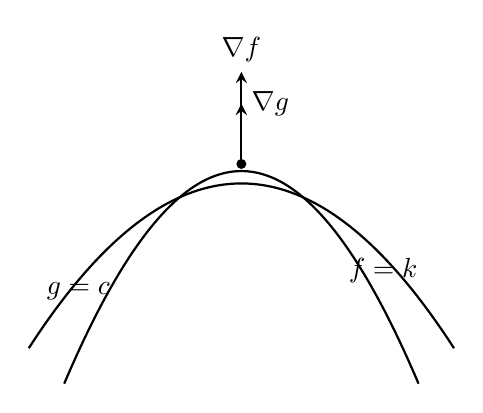
\begin{tikzpicture}[scale=0.9,>=stealth]
\draw[thick] (-3,-1.4) .. controls (-1,1.7) and (1,1.7) .. (3,-1.4);
\draw[thick] (-2.5,-1.9) .. controls (-0.8,2.1) and (0.8,2.1) .. (2.5,-1.9);
\fill (0,1.2) circle (2pt);
\draw[->,thick] (0,1.2)--(0,2.5) node[above] {$\nabla f$};
\draw[->,thick] (0,1.2)--(0,2.05) node[right] {$\nabla g$};
\node at (-2.3,-0.6) {$g=c$};
\node at (2.0,-0.3) {$f=k$};
\end{tikzpicture}
\end{center}

%%%%%%%%%%%%%%%%%%%%%%%%%%%%%%%%%%%%%%%%%%%%%%%%%%%%%%%%%%%%
\subsection{Worked Example: Lagrange Multipliers}
\label{subsec:worked-lagrange}
%%%%%%%%%%%%%%%%%%%%%%%%%%%%%%%%%%%%%%%%%%%%%%%%%%%%%%%%%%%%

\begin{workedexamplebox}{Optimizing on a Circle}

Find the maximum and minimum values of

\[ f(x,y)=x+y \]

subject to

\[ x^2+y^2=2. \]

\begin{tabularx}{\textwidth}{@{}>{\raggedright\arraybackslash}p{0.42\textwidth}X@{}}
Compute the gradients. &
\(\nabla f=\langle1,1\rangle,\quad
\nabla g=\langle2x,2y\rangle\)\\
Apply \(\nabla f=\lambda\nabla g\). &
\(1=2\lambda x,\quad1=2\lambda y\)\\
Compare the equations. &
\(x=y\)\\
Use the constraint. &
\(2x^2=2\Rightarrow x=\pm1\)\\
Find candidate points. &
\((1,1),\quad(-1,-1)\)\\
Evaluate \(f\). &
\(f(1,1)=2,\quad f(-1,-1)=-2\)
\end{tabularx}

\begin{answerbox}
\[ \boxed{\max f=2,\qquad \min f=-2.} \]
\end{answerbox}
\end{workedexamplebox}

%%%%%%%%%%%%%%%%%%%%%%%%%%%%%%%%%%%%%%%%%%%%%%%%%%%%%%%%%%%%
\subsection{Double Integrals}
\label{subsec:double-integrals}
%%%%%%%%%%%%%%%%%%%%%%%%%%%%%%%%%%%%%%%%%%%%%%%%%%%%%%%%%%%%

Single integrals accumulate over intervals.

Double integrals accumulate over two-dimensional regions.

The notation

\[ \iint_R f(x,y)\,dA \]

is read:

``the double integral over \(R\) of \(f(x,y)\) with respect to area.''

Here

\[ dA \]

represents a small element of area.

If \(f(x,y)\geq0\), then

\[ \iint_R f(x,y)\,dA \]

can represent the volume beneath the surface \(z=f(x,y)\) and above the
region \(R\).

%%%%%%%%%%%%%%%%%%%%%%%%%%%%%%%%%%%%%%%%%%%%%%%%%%%%%%%%%%%%
\subsection{Double Integrals over Rectangles}
\label{subsec:double-integrals-rectangles}
%%%%%%%%%%%%%%%%%%%%%%%%%%%%%%%%%%%%%%%%%%%%%%%%%%%%%%%%%%%%

Suppose

\[ R=[a,b]\times[c,d]. \]

Then, under suitable conditions,

\[ \iint_R f(x,y)\,dA
=
\int_a^b\int_c^d f(x,y)\,dy\,dx. \]

One integrates first with respect to \(y\), then with respect to \(x\).

The order may instead be reversed:

\[ \iint_R f(x,y)\,dA
=
\int_c^d\int_a^b f(x,y)\,dx\,dy. \]

%%%%%%%%%%%%%%%%%%%%%%%%%%%%%%%%%%%%%%%%%%%%%%%%%%%%%%%%%%%%
\subsection{Fubini's Theorem}
\label{subsec:fubini-calculus}
%%%%%%%%%%%%%%%%%%%%%%%%%%%%%%%%%%%%%%%%%%%%%%%%%%%%%%%%%%%%

\begin{theorem}[Fubini's Theorem, Calculus Form]
For a continuous function \(f\) on a rectangle
\[ R=[a,b]\times[c,d], \]
the double integral can be evaluated as either iterated integral:
\[ \iint_R f(x,y)\,dA
=
\int_a^b\int_c^d f(x,y)\,dy\,dx
=
\int_c^d\int_a^b f(x,y)\,dx\,dy. \]
\end{theorem}

More general forms of Fubini's Theorem are developed later in measure and
integration theory.

%%%%%%%%%%%%%%%%%%%%%%%%%%%%%%%%%%%%%%%%%%%%%%%%%%%%%%%%%%%%
\subsection{Worked Example: Double Integral}
\label{subsec:worked-double-integral}
%%%%%%%%%%%%%%%%%%%%%%%%%%%%%%%%%%%%%%%%%%%%%%%%%%%%%%%%%%%%

\begin{workedexamplebox}{Integrating over a Rectangle}

Evaluate

\[ \iint_R(x+2y)\,dA, \qquad
R=[0,1]\times[0,2]. \]

\begin{tabularx}{\textwidth}{@{}>{\raggedright\arraybackslash}p{0.42\textwidth}X@{}}
Write as an iterated integral. &
\(\displaystyle \int_0^1\int_0^2(x+2y)\,dy\,dx\)\\
Integrate with respect to \(y\). &
\(\displaystyle \int_0^1[xy+y^2]_0^2\,dx\)\\
Simplify. &
\(\displaystyle \int_0^1(2x+4)\,dx\)\\
Integrate with respect to \(x\). &
\(\displaystyle [x^2+4x]_0^1=5\)
\end{tabularx}

\begin{answerbox}
\[ \boxed{\iint_R(x+2y)\,dA=5.} \]
\end{answerbox}
\end{workedexamplebox}

%%%%%%%%%%%%%%%%%%%%%%%%%%%%%%%%%%%%%%%%%%%%%%%%%%%%%%%%%%%%
\subsection{General Planar Regions}
\label{subsec:general-planar-regions}
%%%%%%%%%%%%%%%%%%%%%%%%%%%%%%%%%%%%%%%%%%%%%%%%%%%%%%%%%%%%

A region may not be rectangular.

A vertically simple region can be described as

\[ R=\{(x,y):a\leq x\leq b,\ g_1(x)\leq y\leq g_2(x)\}. \]

Then

\[ \iint_R f(x,y)\,dA
=
\int_a^b
\int_{g_1(x)}^{g_2(x)}
f(x,y)\,dy\,dx. \]

A horizontally simple region can be written

\[ R=\{(x,y):c\leq y\leq d,\ h_1(y)\leq x\leq h_2(y)\}. \]

Then

\[ \iint_R f(x,y)\,dA
=
\int_c^d
\int_{h_1(y)}^{h_2(y)}
f(x,y)\,dx\,dy. \]

%%%%%%%%%%%%%%%%%%%%%%%%%%%%%%%%%%%%%%%%%%%%%%%%%%%%%%%%%%%%
\subsection{Describing Regions}
\label{subsec:describing-regions}
%%%%%%%%%%%%%%%%%%%%%%%%%%%%%%%%%%%%%%%%%%%%%%%%%%%%%%%%%%%%

Correctly describing the region is often more difficult than performing the
integration.

For a Type I region, think:

\[ \boxed{\text{left}\leq x\leq\text{right},
\qquad
\text{bottom}\leq y\leq\text{top}.} \]

For a Type II region, think:

\[ \boxed{\text{bottom}\leq y\leq\text{top},
\qquad
\text{left}\leq x\leq\text{right}.} \]

Sketching the region before constructing the integral is usually helpful.

%%%%%%%%%%%%%%%%%%%%%%%%%%%%%%%%%%%%%%%%%%%%%%%%%%%%%%%%%%%%
\subsection{Changing the Order of Integration}
\label{subsec:changing-order-integration}
%%%%%%%%%%%%%%%%%%%%%%%%%%%%%%%%%%%%%%%%%%%%%%%%%%%%%%%%%%%%

An iterated integral may be easier in the opposite order.

Suppose

\[ \int_a^b\int_{g_1(x)}^{g_2(x)}f(x,y)\,dy\,dx \]

is given.

To reverse the order:

\begin{enumerate}
    \item identify the region;
    \item sketch it;
    \item determine the full range of \(y\);
    \item solve the boundary curves for \(x\);
    \item write the new bounds;
    \item integrate in the new order.
\end{enumerate}

Changing order changes the description of the region, not the region itself.

%%%%%%%%%%%%%%%%%%%%%%%%%%%%%%%%%%%%%%%%%%%%%%%%%%%%%%%%%%%%
\subsection{Area from a Double Integral}
\label{subsec:area-double-integral}
%%%%%%%%%%%%%%%%%%%%%%%%%%%%%%%%%%%%%%%%%%%%%%%%%%%%%%%%%%%%

If the integrand is \(1\), then

\[ \iint_R1\,dA \]

measures the area of \(R\).

Thus

\[ \boxed{\operatorname{Area}(R)=\iint_R dA.} \]

This is the two-dimensional analogue of computing length by integrating
\(1\) over an interval.

%%%%%%%%%%%%%%%%%%%%%%%%%%%%%%%%%%%%%%%%%%%%%%%%%%%%%%%%%%%%
\subsection{Average Value over a Region}
\label{subsec:average-value-region}
%%%%%%%%%%%%%%%%%%%%%%%%%%%%%%%%%%%%%%%%%%%%%%%%%%%%%%%%%%%%

If \(R\) has positive area, the average value of \(f\) over \(R\) is

\[ f_{\mathrm{avg}}
=
\frac{1}{\operatorname{Area}(R)}
\iint_R f(x,y)\,dA. \]

This generalizes the single-variable average-value formula

\[ f_{\mathrm{avg}}
=
\frac1{b-a}\int_a^b f(x)\,dx. \]

%%%%%%%%%%%%%%%%%%%%%%%%%%%%%%%%%%%%%%%%%%%%%%%%%%%%%%%%%%%%
\subsection{Mass and Density}
\label{subsec:mass-density-double-integral}
%%%%%%%%%%%%%%%%%%%%%%%%%%%%%%%%%%%%%%%%%%%%%%%%%%%%%%%%%%%%

Suppose a thin lamina occupies a region \(R\) and has density

\[ \rho(x,y). \]

The Greek letter

\[ \rho \]

is rho, pronounced ``row.''

Here it represents mass per unit area.

The total mass is

\[ \boxed{m=\iint_R\rho(x,y)\,dA.} \]

%%%%%%%%%%%%%%%%%%%%%%%%%%%%%%%%%%%%%%%%%%%%%%%%%%%%%%%%%%%%
\subsection{Moments and Center of Mass}
\label{subsec:center-mass-double}
%%%%%%%%%%%%%%%%%%%%%%%%%%%%%%%%%%%%%%%%%%%%%%%%%%%%%%%%%%%%

For a lamina with density \(\rho(x,y)\),

\[ M_x=\iint_R y\rho(x,y)\,dA \]

is the moment about the \(x\)-axis, while

\[ M_y=\iint_R x\rho(x,y)\,dA \]

is the moment about the \(y\)-axis.

The center of mass is

\[ \bar{x}=\frac{M_y}{m},\qquad
\bar{y}=\frac{M_x}{m}. \]

The symbols

\[ \bar{x},\qquad\bar{y} \]

are read ``\(x\)-bar'' and ``\(y\)-bar.''

%%%%%%%%%%%%%%%%%%%%%%%%%%%%%%%%%%%%%%%%%%%%%%%%%%%%%%%%%%%%
\subsection{Polar Coordinates}
\label{subsec:polar-coordinates-multivariable}
%%%%%%%%%%%%%%%%%%%%%%%%%%%%%%%%%%%%%%%%%%%%%%%%%%%%%%%%%%%%

Polar coordinates describe a point in the plane using distance from the
origin and angle.

The coordinate transformation is

\[ x=r\cos\theta,\qquad y=r\sin\theta. \]

Also,

\[ r^2=x^2+y^2. \]

Polar coordinates are especially useful for circular and rotationally
symmetric regions.

%%%%%%%%%%%%%%%%%%%%%%%%%%%%%%%%%%%%%%%%%%%%%%%%%%%%%%%%%%%%
\subsection{Area Element in Polar Coordinates}
\label{subsec:polar-area-element}
%%%%%%%%%%%%%%%%%%%%%%%%%%%%%%%%%%%%%%%%%%%%%%%%%%%%%%%%%%%%

In rectangular coordinates,

\[ dA=dx\,dy. \]

In polar coordinates, a small polar region behaves approximately like a
rectangle with side lengths

\[ dr \]

and

\[ r\,d\theta. \]

Therefore,

\[ \boxed{dA=r\,dr\,d\theta.} \]

\begin{center}
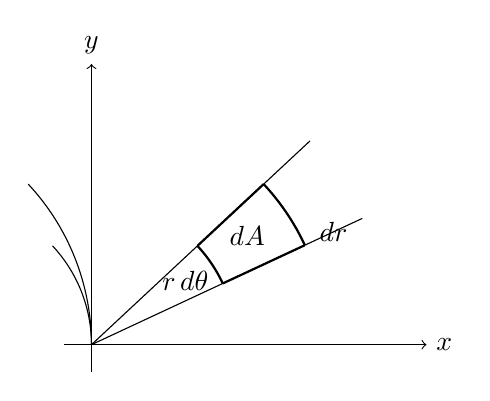
\begin{tikzpicture}[scale=1.15]
\draw[->] (-0.3,0)--(3.7,0) node[right] {$x$};
\draw[->] (0,-0.3)--(0,3.1) node[above] {$y$};

\draw (0,0) -- (25:3.3);
\draw (0,0) -- (43:3.3);

\draw (0,0) arc[start angle=0,end angle=43,radius=1.6];
\draw (0,0) arc[start angle=0,end angle=43,radius=2.6];

\draw[thick] (25:1.6) arc[start angle=25,end angle=43,radius=1.6];
\draw[thick] (25:2.6) arc[start angle=25,end angle=43,radius=2.6];
\draw[thick] (25:1.6)--(25:2.6);
\draw[thick] (43:1.6)--(43:2.6);

\node at (35:2.1) {$dA$};
\node at (34:1.25) {$r\,d\theta$};
\node at (25:2.95) {$dr$};
\end{tikzpicture}
\end{center}

The factor \(r\) is essential.

%%%%%%%%%%%%%%%%%%%%%%%%%%%%%%%%%%%%%%%%%%%%%%%%%%%%%%%%%%%%
\subsection{Double Integrals in Polar Coordinates}
\label{subsec:double-integrals-polar}
%%%%%%%%%%%%%%%%%%%%%%%%%%%%%%%%%%%%%%%%%%%%%%%%%%%%%%%%%%%%

A double integral may be transformed using

\[ x=r\cos\theta,\qquad y=r\sin\theta,\qquad dA=r\,dr\,d\theta. \]

Thus

\[ \boxed{
\iint_R f(x,y)\,dA
=
\iint_S
f(r\cos\theta,r\sin\theta)\,r\,dr\,d\theta.
} \]

Here \(S\) is the corresponding region in the \(r\theta\)-coordinate plane.

%%%%%%%%%%%%%%%%%%%%%%%%%%%%%%%%%%%%%%%%%%%%%%%%%%%%%%%%%%%%
\subsection{Worked Example: Polar Integration}
\label{subsec:worked-polar-integration}
%%%%%%%%%%%%%%%%%%%%%%%%%%%%%%%%%%%%%%%%%%%%%%%%%%%%%%%%%%%%

\begin{workedexamplebox}{Area of a Disk}

Use a double integral to find the area of the disk

\[ x^2+y^2\leq R^2. \]

\begin{tabularx}{\textwidth}{@{}>{\raggedright\arraybackslash}p{0.42\textwidth}X@{}}
Use polar coordinates. &
\(0\leq r\leq R,\quad0\leq\theta\leq2\pi\)\\
Use \(dA=r\,dr\,d\theta\). &
\(\displaystyle A=\int_0^{2\pi}\int_0^R r\,dr\,d\theta\)\\
Integrate with respect to \(r\). &
\(\displaystyle \int_0^{2\pi}\frac{R^2}{2}\,d\theta\)\\
Integrate with respect to \(\theta\). &
\(\displaystyle \frac{R^2}{2}(2\pi)=\pi R^2\)
\end{tabularx}

\begin{answerbox}
\[ \boxed{A=\pi R^2.} \]
\end{answerbox}
\end{workedexamplebox}

%%%%%%%%%%%%%%%%%%%%%%%%%%%%%%%%%%%%%%%%%%%%%%%%%%%%%%%%%%%%
\subsection{Triple Integrals}
\label{subsec:triple-integrals}
%%%%%%%%%%%%%%%%%%%%%%%%%%%%%%%%%%%%%%%%%%%%%%%%%%%%%%%%%%%%

Triple integrals accumulate quantities over three-dimensional regions.

The notation

\[ \iiint_E f(x,y,z)\,dV \]

is read:

``the triple integral over \(E\) of \(f(x,y,z)\) with respect to volume.''

Here

\[ dV \]

represents a small volume element.

For example,

\[ \iiint_E1\,dV \]

gives the volume of \(E\).

%%%%%%%%%%%%%%%%%%%%%%%%%%%%%%%%%%%%%%%%%%%%%%%%%%%%%%%%%%%%
\subsection{Triple Integrals in Rectangular Coordinates}
\label{subsec:triple-rectangular}
%%%%%%%%%%%%%%%%%%%%%%%%%%%%%%%%%%%%%%%%%%%%%%%%%%%%%%%%%%%%

In Cartesian coordinates,

\[ dV=dx\,dy\,dz \]

up to the chosen order of integration.

For a rectangular box

\[ E=[a,b]\times[c,d]\times[p,q], \]

one possible iterated integral is

\[ \iiint_Ef\,dV
=
\int_a^b\int_c^d\int_p^q
f(x,y,z)\,dz\,dy\,dx. \]

Under suitable conditions, the order of integration may be changed.

%%%%%%%%%%%%%%%%%%%%%%%%%%%%%%%%%%%%%%%%%%%%%%%%%%%%%%%%%%%%
\subsection{Volume from Triple Integrals}
\label{subsec:volume-triple-integral}
%%%%%%%%%%%%%%%%%%%%%%%%%%%%%%%%%%%%%%%%%%%%%%%%%%%%%%%%%%%%

The volume of a three-dimensional region \(E\) is

\[ \boxed{\operatorname{Vol}(E)=\iiint_E dV.} \]

If the region contains material with density

\[ \rho(x,y,z), \]

its mass is

\[ m=\iiint_E\rho(x,y,z)\,dV. \]

%%%%%%%%%%%%%%%%%%%%%%%%%%%%%%%%%%%%%%%%%%%%%%%%%%%%%%%%%%%%
\subsection{Cylindrical Coordinates}
\label{subsec:cylindrical-coordinates}
%%%%%%%%%%%%%%%%%%%%%%%%%%%%%%%%%%%%%%%%%%%%%%%%%%%%%%%%%%%%

Cylindrical coordinates extend polar coordinates into three dimensions.

The transformation is

\[ x=r\cos\theta,\qquad y=r\sin\theta,\qquad z=z. \]

The volume element is

\[ \boxed{dV=r\,dr\,d\theta\,dz} \]

up to the chosen integration order.

Cylindrical coordinates are useful for solids with symmetry around an axis.

%%%%%%%%%%%%%%%%%%%%%%%%%%%%%%%%%%%%%%%%%%%%%%%%%%%%%%%%%%%%
\subsection{Spherical Coordinates}
\label{subsec:spherical-coordinates}
%%%%%%%%%%%%%%%%%%%%%%%%%%%%%%%%%%%%%%%%%%%%%%%%%%%%%%%%%%%%

Spherical coordinates describe a point using a radial distance and two
angles.

A common convention is

\[ x=\rho\sin\phi\cos\theta, \]

\[ y=\rho\sin\phi\sin\theta, \]

\[ z=\rho\cos\phi. \]

The Greek letter

\[ \phi \]

is phi, commonly pronounced ``fie'' or ``fee.''

In this convention:

\begin{itemize}
    \item \(\rho\geq0\) is distance from the origin;
    \item \(\theta\) is the azimuthal angle in the \(xy\)-plane;
    \item \(\phi\) is the angle measured downward from the positive \(z\)-axis.
\end{itemize}

%%%%%%%%%%%%%%%%%%%%%%%%%%%%%%%%%%%%%%%%%%%%%%%%%%%%%%%%%%%%
\subsection{Spherical Volume Element}
\label{subsec:spherical-volume-element}
%%%%%%%%%%%%%%%%%%%%%%%%%%%%%%%%%%%%%%%%%%%%%%%%%%%%%%%%%%%%

The spherical-coordinate volume element is

\[ \boxed{
dV=\rho^2\sin\phi\,d\rho\,d\phi\,d\theta.
} \]

The factor

\[ \rho^2\sin\phi \]

accounts for the geometric distortion caused by the coordinate
transformation.

For a sphere of radius \(R\), typical bounds are

\[ 0\leq\rho\leq R,\qquad
0\leq\phi\leq\pi,\qquad
0\leq\theta\leq2\pi. \]

%%%%%%%%%%%%%%%%%%%%%%%%%%%%%%%%%%%%%%%%%%%%%%%%%%%%%%%%%%%%
\subsection{Worked Example: Volume of a Sphere}
\label{subsec:worked-sphere-volume}
%%%%%%%%%%%%%%%%%%%%%%%%%%%%%%%%%%%%%%%%%%%%%%%%%%%%%%%%%%%%

\begin{workedexamplebox}{Volume Using Spherical Coordinates}

Find the volume of a sphere of radius \(R\).

\begin{tabularx}{\textwidth}{@{}>{\raggedright\arraybackslash}p{0.42\textwidth}X@{}}
Write the bounds. &
\(0\leq\rho\leq R,\ 0\leq\phi\leq\pi,\ 0\leq\theta\leq2\pi\)\\
Use the spherical volume element. &
\(\displaystyle V=\int_0^{2\pi}\int_0^\pi\int_0^R
\rho^2\sin\phi\,d\rho\,d\phi\,d\theta\)\\
Integrate in \(\rho\). &
\(\displaystyle \frac{R^3}{3}\)\\
Integrate in \(\phi\). &
\(\displaystyle \int_0^\pi\sin\phi\,d\phi=2\)\\
Integrate in \(\theta\). &
\(\displaystyle \int_0^{2\pi}d\theta=2\pi\)
\end{tabularx}

\begin{answerbox}
\[ \boxed{V=\frac43\pi R^3.} \]
\end{answerbox}
\end{workedexamplebox}

%%%%%%%%%%%%%%%%%%%%%%%%%%%%%%%%%%%%%%%%%%%%%%%%%%%%%%%%%%%%
\subsection{Change of Variables}
\label{subsec:change-of-variables-multivariable}
%%%%%%%%%%%%%%%%%%%%%%%%%%%%%%%%%%%%%%%%%%%%%%%%%%%%%%%%%%%%

Substitution in one-dimensional integration changes one variable into
another.

Multivariable integration allows simultaneous coordinate transformations.

Suppose

\[ x=x(u,v),\qquad y=y(u,v). \]

Then area is distorted by a scale factor determined by the derivatives of
the transformation.

This scale factor is described by a Jacobian determinant.

%%%%%%%%%%%%%%%%%%%%%%%%%%%%%%%%%%%%%%%%%%%%%%%%%%%%%%%%%%%%
\subsection{The Jacobian Matrix}
\label{subsec:jacobian-matrix}
%%%%%%%%%%%%%%%%%%%%%%%%%%%%%%%%%%%%%%%%%%%%%%%%%%%%%%%%%%%%

For the transformation

\[ T(u,v)=\langle x(u,v),y(u,v)\rangle, \]

the derivative information can be organized into the matrix

\[ DT=
\begin{pmatrix}
\dfrac{\partial x}{\partial u} &
\dfrac{\partial x}{\partial v}\\[2mm]
\dfrac{\partial y}{\partial u} &
\dfrac{\partial y}{\partial v}
\end{pmatrix}. \]

This matrix is called the \emph{Jacobian matrix} of the transformation.

It represents the best local linear approximation to \(T\).

%%%%%%%%%%%%%%%%%%%%%%%%%%%%%%%%%%%%%%%%%%%%%%%%%%%%%%%%%%%%
\subsection{Jacobian Determinant}
\label{subsec:jacobian-determinant}
%%%%%%%%%%%%%%%%%%%%%%%%%%%%%%%%%%%%%%%%%%%%%%%%%%%%%%%%%%%%

The determinant

\[ \frac{\partial(x,y)}{\partial(u,v)}
=
\begin{vmatrix}
x_u & x_v\\
y_u & y_v
\end{vmatrix} \]

is called the \emph{Jacobian determinant}.

The notation

\[ \frac{\partial(x,y)}{\partial(u,v)} \]

is read:

``the Jacobian of \(x,y\) with respect to \(u,v\).''

Its absolute value measures local area scaling.

%%%%%%%%%%%%%%%%%%%%%%%%%%%%%%%%%%%%%%%%%%%%%%%%%%%%%%%%%%%%
\subsection{Change-of-Variables Formula}
\label{subsec:change-variables-formula}
%%%%%%%%%%%%%%%%%%%%%%%%%%%%%%%%%%%%%%%%%%%%%%%%%%%%%%%%%%%%

Under appropriate hypotheses,

\[ \boxed{
\iint_R f(x,y)\,dx\,dy
=
\iint_S
f(x(u,v),y(u,v))
\left|
\frac{\partial(x,y)}{\partial(u,v)}
\right|
\,du\,dv.
} \]

The absolute value appears because area is nonnegative regardless of
orientation.

%%%%%%%%%%%%%%%%%%%%%%%%%%%%%%%%%%%%%%%%%%%%%%%%%%%%%%%%%%%%
\subsection{Polar Coordinates as a Jacobian}
\label{subsec:polar-jacobian}
%%%%%%%%%%%%%%%%%%%%%%%%%%%%%%%%%%%%%%%%%%%%%%%%%%%%%%%%%%%%

For polar coordinates,

\[ x=r\cos\theta,\qquad y=r\sin\theta. \]

The Jacobian is

\[
\frac{\partial(x,y)}{\partial(r,\theta)}
=
\begin{vmatrix}
\cos\theta & -r\sin\theta\\
\sin\theta & r\cos\theta
\end{vmatrix}.
\]

Therefore,

\[ \frac{\partial(x,y)}{\partial(r,\theta)}
=r\cos^2\theta+r\sin^2\theta=r. \]

Hence

\[ dA=r\,dr\,d\theta. \]

Thus the familiar polar-coordinate factor \(r\) is not an arbitrary rule;
it is a Jacobian determinant.

%%%%%%%%%%%%%%%%%%%%%%%%%%%%%%%%%%%%%%%%%%%%%%%%%%%%%%%%%%%%
\subsection{Worked Example: Change of Variables}
\label{subsec:worked-change-variables}
%%%%%%%%%%%%%%%%%%%%%%%%%%%%%%%%%%%%%%%%%%%%%%%%%%%%%%%%%%%%

\begin{workedexamplebox}{A Linear Coordinate Transformation}

Let

\[ x=u+v,\qquad y=u-v. \]

Find the area scaling factor.

\begin{tabularx}{\textwidth}{@{}>{\raggedright\arraybackslash}p{0.42\textwidth}X@{}}
Compute the derivatives. &
\(x_u=1,\ x_v=1,\ y_u=1,\ y_v=-1\)\\
Form the Jacobian. &
\(\displaystyle
\frac{\partial(x,y)}{\partial(u,v)}
=
\begin{vmatrix}
1&1\\
1&-1
\end{vmatrix}\)\\
Evaluate the determinant. &
\(-1-1=-2\)\\
Take the absolute value. &
\(2\)
\end{tabularx}

\begin{answerbox}
\[ \boxed{dA=2\,du\,dv.} \]
\end{answerbox}
\end{workedexamplebox}

%%%%%%%%%%%%%%%%%%%%%%%%%%%%%%%%%%%%%%%%%%%%%%%%%%%%%%%%%%%%
\subsection{Higher-Dimensional Viewpoint}
\label{subsec:higher-dimensional-multivariable}
%%%%%%%%%%%%%%%%%%%%%%%%%%%%%%%%%%%%%%%%%%%%%%%%%%%%%%%%%%%%

The ideas of multivariable calculus extend naturally to

\[ f:\R^n\to\R^m. \]

For scalar-valued functions

\[ f:\R^n\to\R, \]

the gradient contains first-order derivative information.

For vector-valued functions

\[ F:\R^n\to\R^m, \]

the first derivatives are organized into a Jacobian matrix.

Thus the single derivative number

\[ f'(a) \]

from one-variable calculus becomes a linear transformation in higher
dimensions.

%%%%%%%%%%%%%%%%%%%%%%%%%%%%%%%%%%%%%%%%%%%%%%%%%%%%%%%%%%%%
\subsection{Derivative as a Linear Map}
\label{subsec:derivative-linear-map}
%%%%%%%%%%%%%%%%%%%%%%%%%%%%%%%%%%%%%%%%%%%%%%%%%%%%%%%%%%%%

For a differentiable map

\[ F:\R^n\to\R^m, \]

the derivative at a point \(\vect{a}\) is the linear transformation that best
approximates \(F\) near \(\vect{a}\).

Informally,

\[ F(\vect{a}+\vect{h})
\approx
F(\vect{a})+DF(\vect{a})\vect{h}. \]

This viewpoint unifies:

\begin{itemize}
    \item ordinary derivatives;
    \item gradients;
    \item tangent planes;
    \item Jacobian matrices;
    \item directional derivatives;
    \item the multivariable chain rule.
\end{itemize}

\begin{conceptbox}
The deepest interpretation of multivariable differentiation is not
``taking many partial derivatives.'' It is finding the best local linear
approximation to a function.
\end{conceptbox}

%%%%%%%%%%%%%%%%%%%%%%%%%%%%%%%%%%%%%%%%%%%%%%%%%%%%%%%%%%%%
\subsection{Applications}
\label{subsec:multivariable-applications}
%%%%%%%%%%%%%%%%%%%%%%%%%%%%%%%%%%%%%%%%%%%%%%%%%%%%%%%%%%%%

\begin{applicationbox}
\textbf{Physics.}
Temperature, pressure, gravitational potential, electric potential, and
density naturally depend on several spatial variables. Gradients describe
directions of strongest change, while multiple integrals compute mass,
charge, energy, and other accumulated quantities.

\medskip

\textbf{Engineering.}
Multivariable calculus appears in thermodynamics, mechanics, control,
electromagnetism, fluid systems, optimization, and numerical simulation.

\medskip

\textbf{Environmental Science.}
Temperature, dissolved oxygen, pollution concentration, rainfall, elevation,
and other measurements may vary simultaneously across location, depth, and
time.

\medskip

\textbf{Economics.}
Production and utility functions often depend on several inputs. Partial
derivatives represent marginal changes while constrained optimization
models limited resources.

\medskip

\textbf{Statistics.}
Likelihood functions depend on multiple parameters. Gradients and Hessians
play central roles in estimation and numerical optimization.

\medskip

\textbf{Machine Learning.}
A loss function may depend on thousands or millions of parameters.
Gradient-based optimization adjusts those parameters in directions that
reduce the loss.

\medskip

\textbf{Geometry.}
Level sets, tangent spaces, Jacobians, and local linearization form a bridge
from calculus to differential geometry.

\medskip

\textbf{Differential Equations.}
Partial derivatives are the fundamental language of partial differential
equations, where unknown functions depend on several variables.
\end{applicationbox}

%%%%%%%%%%%%%%%%%%%%%%%%%%%%%%%%%%%%%%%%%%%%%%%%%%%%%%%%%%%%
\subsection{Common Errors}
\label{subsec:multivariable-common-errors}
%%%%%%%%%%%%%%%%%%%%%%%%%%%%%%%%%%%%%%%%%%%%%%%%%%%%%%%%%%%%

\subsubsection{Checking Only One Path}

A single path can never establish a multivariable limit.

Different paths may produce different behavior.

%%%%%%%%%%%%%%%%%%%%%%%%%%%%%%%%%%%%%%%%%%%%%%%%%%%%%%%%%%%%
\subsubsection{Assuming Many Matching Paths Prove a Limit}

Even if several paths produce the same value, another path may behave
differently.

A proof of existence requires stronger reasoning.

%%%%%%%%%%%%%%%%%%%%%%%%%%%%%%%%%%%%%%%%%%%%%%%%%%%%%%%%%%%%
\subsubsection{Differentiating Every Variable in a Partial Derivative}

When computing

\[ f_x, \]

all variables other than \(x\) are treated as constants.

%%%%%%%%%%%%%%%%%%%%%%%%%%%%%%%%%%%%%%%%%%%%%%%%%%%%%%%%%%%%
\subsubsection{Assuming Partial Derivatives Guarantee Differentiability}

The existence of

\[ f_x(a,b),\qquad f_y(a,b) \]

does not by itself imply differentiability.

%%%%%%%%%%%%%%%%%%%%%%%%%%%%%%%%%%%%%%%%%%%%%%%%%%%%%%%%%%%%
\subsubsection{Using a Nonunit Direction Vector}

The formula

\[ D_{\vect{u}}f=\nabla f\cdot\vect{u} \]

assumes

\[ \norm{\vect{u}}=1. \]

Normalize the direction vector first.

%%%%%%%%%%%%%%%%%%%%%%%%%%%%%%%%%%%%%%%%%%%%%%%%%%%%%%%%%%%%
\subsubsection{Confusing Gradient with Directional Derivative}

The gradient

\[ \nabla f \]

is a vector.

The directional derivative

\[ D_{\vect{u}}f \]

is a scalar.

%%%%%%%%%%%%%%%%%%%%%%%%%%%%%%%%%%%%%%%%%%%%%%%%%%%%%%%%%%%%
\subsubsection{Ignoring the Constraint in Lagrange Multipliers}

Solving only

\[ \nabla f=\lambda\nabla g \]

is incomplete.

The constraint equation

\[ g(x,y)=c \]

must also be satisfied.

%%%%%%%%%%%%%%%%%%%%%%%%%%%%%%%%%%%%%%%%%%%%%%%%%%%%%%%%%%%%
\subsubsection{Using the Hessian Test When \(D=0\)}

If

\[ D=0, \]

the second derivative test is inconclusive.

Another method must be used.

%%%%%%%%%%%%%%%%%%%%%%%%%%%%%%%%%%%%%%%%%%%%%%%%%%%%%%%%%%%%
\subsubsection{Reading Iterated Integrals in the Wrong Order}

In

\[ \int_a^b\int_c^d f(x,y)\,dy\,dx, \]

the \(y\)-integration is performed first.

%%%%%%%%%%%%%%%%%%%%%%%%%%%%%%%%%%%%%%%%%%%%%%%%%%%%%%%%%%%%
\subsubsection{Incorrect Region Bounds}

Bounds must describe the actual geometric region.

Sketching the region can prevent many setup errors.

%%%%%%%%%%%%%%%%%%%%%%%%%%%%%%%%%%%%%%%%%%%%%%%%%%%%%%%%%%%%
\subsubsection{Forgetting the Polar Jacobian}

In polar coordinates,

\[ dA\neq dr\,d\theta. \]

The correct area element is

\[ dA=r\,dr\,d\theta. \]

%%%%%%%%%%%%%%%%%%%%%%%%%%%%%%%%%%%%%%%%%%%%%%%%%%%%%%%%%%%%
\subsubsection{Forgetting the Spherical Jacobian}

In spherical coordinates,

\[ dV\neq d\rho\,d\phi\,d\theta. \]

Instead,

\[ dV=\rho^2\sin\phi\,d\rho\,d\phi\,d\theta. \]

%%%%%%%%%%%%%%%%%%%%%%%%%%%%%%%%%%%%%%%%%%%%%%%%%%%%%%%%%%%%
\subsubsection{Ignoring the Absolute Value of a Jacobian}

In change-of-variables formulas, area and volume scaling use

\[ \left|\det J\right|. \]

The absolute value is essential.

%%%%%%%%%%%%%%%%%%%%%%%%%%%%%%%%%%%%%%%%%%%%%%%%%%%%%%%%%%%%
\subsection{Exercises}
\label{subsec:multivariable-exercises}
%%%%%%%%%%%%%%%%%%%%%%%%%%%%%%%%%%%%%%%%%%%%%%%%%%%%%%%%%%%%

\begin{exercise}[1]
Find the domain of
\[ f(x,y)=\sqrt{16-x^2-y^2}. \]
\end{exercise}

\begin{exercise}[1]
Describe the level curves of
\[ f(x,y)=x^2+4y^2. \]
\end{exercise}

\begin{exercise}[2]
Describe the traces of
\[ z=x^2-y^2 \]
in the planes \(x=0\), \(y=0\), and \(z=0\).
\end{exercise}

\begin{exercise}[2]
Determine whether
\[ \lim_{(x,y)\to(0,0)}
\frac{x^2-y^2}{x^2+y^2} \]
exists.
\end{exercise}

\begin{exercise}[2]
Evaluate
\[ \lim_{(x,y)\to(0,0)}
\frac{x^2y}{x^2+y^2}. \]
\end{exercise}

\begin{exercise}[2]
Use polar coordinates to evaluate
\[ \lim_{(x,y)\to(0,0)}
\frac{x^4+y^4}{x^2+y^2}. \]
\end{exercise}

\begin{exercise}[1]
For
\[ f(x,y)=x^2y+xy^3, \]
find \(f_x\) and \(f_y\).
\end{exercise}

\begin{exercise}[2]
For
\[ f(x,y)=e^{xy}\sin x, \]
find \(f_x\) and \(f_y\).
\end{exercise}

\begin{exercise}[2]
Find
\[ f_{xx},\quad f_{xy},\quad f_{yx},\quad f_{yy} \]
for
\[ f(x,y)=x^3y^2. \]
\end{exercise}

\begin{exercise}[2]
Find the tangent plane to
\[ z=x^2+2y^2 \]
at \((1,1,3)\).
\end{exercise}

\begin{exercise}[2]
Find the linearization of
\[ f(x,y)=\sqrt{x+y} \]
at \((2,2)\).
\end{exercise}

\begin{exercise}[2]
Use differentials to approximate the change in
\[ f(x,y)=x^2y \]
when \(x\) changes from \(2\) to \(2.01\) and \(y\) changes from \(3\) to
\(2.98\).
\end{exercise}

\begin{exercise}[1]
Find the gradient of
\[ f(x,y)=x^2+y^2. \]
\end{exercise}

\begin{exercise}[2]
Find the directional derivative of
\[ f(x,y)=x^2y \]
at \((1,2)\) in the direction of
\[ \vect{v}=\langle1,1\rangle. \]
\end{exercise}

\begin{exercise}[2]
For
\[ f(x,y)=x^2+4y^2, \]
find the direction of maximum increase at \((2,1)\).
\end{exercise}

\begin{exercise}[2]
Find the maximum rate of increase of
\[ f(x,y)=xe^y \]
at \((1,0)\).
\end{exercise}

\begin{exercise}[2]
Show that the gradient of
\[ f(x,y)=x^2+y^2 \]
is perpendicular to its circular level curves.
\end{exercise}

\begin{exercise}[2]
Let
\[ z=x^2y,\qquad x=t^2,\qquad y=e^t. \]
Find \(dz/dt\).
\end{exercise}

\begin{exercise}[2]
Suppose
\[ z=x^2+y^2,\qquad x=s+t,\qquad y=s-t. \]
Find
\[ \frac{\partial z}{\partial s}
\qquad\text{and}\qquad
\frac{\partial z}{\partial t}. \]
\end{exercise}

\begin{exercise}[2]
If
\[ x^2+xy+y^2=7, \]
use the multivariable implicit formula to find \(dy/dx\).
\end{exercise}

\begin{exercise}[1]
Find the critical points of
\[ f(x,y)=x^2+y^2-4x+6y. \]
\end{exercise}

\begin{exercise}[2]
Classify the critical point of
\[ f(x,y)=x^2-y^2. \]
\end{exercise}

\begin{exercise}[2]
Classify all critical points of
\[ f(x,y)=x^3-3x+y^2. \]
\end{exercise}

\begin{exercise}[2]
Find the absolute maximum and minimum of
\[ f(x,y)=x^2+y^2 \]
on the disk
\[ x^2+y^2\leq4. \]
\end{exercise}

\begin{exercise}[2]
Use Lagrange multipliers to maximize and minimize
\[ f(x,y)=xy \]
subject to
\[ x^2+y^2=2. \]
\end{exercise}

\begin{exercise}[3]
Use Lagrange multipliers to find the point on
\[ x^2+4y^2=4 \]
that maximizes \(x+y\).
\end{exercise}

\begin{exercise}[1]
Evaluate
\[ \int_0^1\int_0^2(x+y)\,dy\,dx. \]
\end{exercise}

\begin{exercise}[2]
Evaluate
\[ \iint_Rxy\,dA \]
where
\[ R=[0,2]\times[1,3]. \]
\end{exercise}

\begin{exercise}[2]
Set up a double integral for the region bounded by
\[ y=x^2 \]
and
\[ y=x. \]
\end{exercise}

\begin{exercise}[2]
Reverse the order of integration in
\[ \int_0^1\int_x^1 f(x,y)\,dy\,dx. \]
\end{exercise}

\begin{exercise}[2]
Use a double integral to find the area of
\[ R=\{(x,y):0\leq x\leq2,\ 0\leq y\leq x^2\}. \]
\end{exercise}

\begin{exercise}[2]
Find the average value of
\[ f(x,y)=x+y \]
over the unit square.
\end{exercise}

\begin{exercise}[2]
A lamina occupies the unit square and has density
\[ \rho(x,y)=x+y+1. \]
Find its mass.
\end{exercise}

\begin{exercise}[3]
For the lamina in the previous exercise, find its center of mass.
\end{exercise}

\begin{exercise}[2]
Use polar coordinates to evaluate
\[ \iint_R(x^2+y^2)\,dA, \]
where \(R\) is the unit disk.
\end{exercise}

\begin{exercise}[2]
Use polar coordinates to find the area inside
\[ x^2+y^2=9. \]
\end{exercise}

\begin{exercise}[2]
Evaluate
\[ \iiint_E1\,dV \]
for
\[ E=[0,1]\times[0,2]\times[0,3]. \]
\end{exercise}

\begin{exercise}[2]
Use cylindrical coordinates to find the volume of a cylinder of radius
\(R\) and height \(h\).
\end{exercise}

\begin{exercise}[2]
Use spherical coordinates to verify the volume formula
\[ V=\frac43\pi R^3. \]
\end{exercise}

\begin{exercise}[2]
Find the Jacobian determinant for
\[ x=2u+v,\qquad y=u-3v. \]
\end{exercise}

\begin{exercise}[2]
Verify directly that the polar-coordinate Jacobian is \(r\).
\end{exercise}

\begin{exercise}[3]
Use the transformation
\[ u=x+y,\qquad v=x-y \]
to describe how area elements transform.
\end{exercise}

\begin{exercise}[3]
Let
\[ f(x,y)=x^4+y^4-4xy. \]
Find and classify all critical points.
\end{exercise}

\begin{exercise}[3]
Find the extrema of
\[ f(x,y,z)=x+y+z \]
subject to
\[ x^2+y^2+z^2=1. \]
\end{exercise}

%%%%%%%%%%%%%%%%%%%%%%%%%%%%%%%%%%%%%%%%%%%%%%%%%%%%%%%%%%%%
\subsection{Conceptual Summary}
\label{subsec:multivariable-summary}
%%%%%%%%%%%%%%%%%%%%%%%%%%%%%%%%%%%%%%%%%%%%%%%%%%%%%%%%%%%%

Multivariable calculus extends the central ideas of calculus into higher
dimensions.

A function such as

\[ f(x,y) \]

can be visualized through surfaces and level curves.

Limits now require consistent behavior along all approaches to a point.

Partial derivatives measure coordinate-direction change:

\[ f_x,\qquad f_y. \]

The gradient collects these derivatives:

\[ \nabla f=\langle f_x,f_y\rangle. \]

Directional derivatives satisfy

\[ D_{\vect{u}}f=\nabla f\cdot\vect{u}. \]

Differentiability leads to the local linear approximation

\[ f(a+\Delta x,b+\Delta y)
\approx
f(a,b)+f_x\Delta x+f_y\Delta y. \]

Second derivatives form the Hessian and reveal local curvature.

Optimization extends to several variables through critical-point analysis and
Lagrange multipliers:

\[ \nabla f=\lambda\nabla g. \]

Integration extends from intervals to regions and solids:

\[ \int_a^b f(x)\,dx
\quad\longrightarrow\quad
\iint_R f(x,y)\,dA
\quad\longrightarrow\quad
\iiint_E f(x,y,z)\,dV. \]

Coordinate transformations require Jacobian scaling:

\[ dA=
\left|
\frac{\partial(x,y)}{\partial(u,v)}
\right|du\,dv. \]

\begin{center}
\begin{tikzpicture}[
    node distance=11mm and 14mm,
    box/.style={draw,rounded corners,align=center,inner sep=5pt},
    >=stealth
]
\node[box] (func) {Multivariable\\functions};
\node[box,below left=of func] (diff) {Differentiation};
\node[box,below right=of func] (int) {Integration};
\node[box,below=of diff] (grad) {Gradient\\Hessian};
\node[box,below=of int] (multi) {Double and\\triple integrals};
\node[box,below=of grad] (opt) {Optimization};
\node[box,below=of multi] (coord) {Coordinate\\transformations};

\draw[->] (func)--(diff);
\draw[->] (func)--(int);
\draw[->] (diff)--(grad);
\draw[->] (int)--(multi);
\draw[->] (grad)--(opt);
\draw[->] (multi)--(coord);
\end{tikzpicture}
\end{center}

%%%%%%%%%%%%%%%%%%%%%%%%%%%%%%%%%%%%%%%%%%%%%%%%%%%%%%%%%%%%
\subsection{Section Connections}
\label{subsec:multivariable-connections}
%%%%%%%%%%%%%%%%%%%%%%%%%%%%%%%%%%%%%%%%%%%%%%%%%%%%%%%%%%%%

\chapterconnection{
Multivariable calculus extends the limit, derivative, optimization, and
integration concepts of single-variable calculus to functions defined on
higher-dimensional spaces. Partial derivatives measure coordinate changes,
while the gradient describes the complete first-order behavior of a
scalar-valued function. Differentiability is best understood through local
linear approximation, connecting calculus directly to linear algebra.
Hessian matrices encode second-order behavior and support multivariable
optimization. Multiple integrals extend accumulation from intervals to
regions and solids, while Jacobian determinants explain how area and volume
change under coordinate transformations. These ideas provide the immediate
foundation for vector calculus, differential geometry, partial differential
equations, optimization, probability, statistics, mathematical physics, and
the higher-dimensional theories developed in Real and Functional Analysis.
}

%%%%%%%%%%%%%%%%%%%%%%%%%%%%%%%%%%%%%%%%%%%%%%%%%%%%%%%%%%%%
% SECTION SOURCE TRACKING
%%%%%%%%%%%%%%%%%%%%%%%%%%%%%%%%%%%%%%%%%%%%%%%%%%%%%%%%%%%%

%------------------------------------------------------------
% 5.3 Multivariable Calculus
%------------------------------------------------------------
%
% Sources:
%   - This section uses standard undergraduate multivariable-calculus theory
%     together with the single-variable calculus, function, and linear
%     algebra foundations established earlier in the text.
%
% Used for:
%   - functions of several variables;
%   - surfaces, traces, level curves, and level surfaces;
%   - multivariable limits and continuity;
%   - partial derivatives;
%   - tangent planes and linearization;
%   - gradients and directional derivatives;
%   - multivariable chain rules;
%   - Hessian matrices;
%   - unconstrained optimization;
%   - Lagrange multipliers;
%   - double and triple integration;
%   - polar, cylindrical, and spherical coordinates;
%   - mass, center of mass, and average value;
%   - Jacobian matrices and change of variables.
%
% Notes:
%   - Vector algebra and linear transformations are taught canonically in
%     Linear Algebra.
%   - Single-variable limits, derivatives, and integrals are taught
%     canonically in Single-Variable Calculus.
%   - Vector fields, line integrals, surface integrals, divergence, curl,
%     Green's Theorem, Stokes' Theorem, and the Divergence Theorem belong
%     canonically to Vector Calculus.
%   - Formal higher-dimensional limit and differentiability theory is
%     developed later in Real Analysis.
%   - General Fubini and change-of-variables theorems are revisited with
%     greater rigor in Measure Theory and Lebesgue Integration.
%   - Manifolds and coordinate charts belong canonically to Differential
%     Geometry and Manifold Theory.
%   - Partial differential equations are developed in the Differential
%     Equations branch.
%   - Visualizations and pedagogical organization are independently
%     developed for this text.